\documentclass[a4paper,twoside,titlepage,11pt,floatssmall]{mwrep}
\usepackage[inner=3.0cm,outer=2.0cm,top=2.5cm,bottom=2.5cm]{geometry}
\usepackage[OT1]{fontenc}
\usepackage{polski}
\usepackage{amsmath}
\usepackage{amsfonts}
\usepackage{amssymb}
\usepackage{setspace}
\usepackage{graphicx}
\usepackage{float}
\usepackage{subfig}
\usepackage{url}
\usepackage{tikz}
\usetikzlibrary{arrows,calc,decorations.markings,math,arrows.meta}
\usepackage{rotating}
\usepackage[percent]{overpic}
\usepackage[utf8]{inputenc}
\usepackage{xcolor}
\usepackage{colortbl}
\usepackage{listings}
\usepackage{matlab-prettifier}
\usepackage{enumitem,amssymb}
\definecolor{szary}{rgb}{0.95,0.95,0.95}
\usepackage{siunitx}
\sisetup{detect-weight,exponent-product=\cdot,output-decimal-marker={,},per-mode=symbol,range-phrase={-},range-units=single}

%konfiguracje pakietu listings
\lstset{
  literate={ą}{{\k a}}1
           {Ą}{{\k A}}1
           {ż}{{\. z}}1
           {Ż}{{\. Z}}1
           {ź}{{\' z}}1
           {Ź}{{\' Z}}1
           {ć}{{\' c}}1
           {Ć}{{\' C}}1
           {ę}{{\k e}}1
           {Ę}{{\k E}}1
           {ó}{{\' o}}1
           {Ó}{{\' O}}1
           {ń}{{\' n}}1
           {Ń}{{\' N}}1
           {ś}{{\' s}}1
           {Ś}{{\' S}}1
           {ł}{{\l}}1
           {Ł}{{\L}}1
}
\lstset{
	backgroundcolor=\color{szary},
	frame=single,
	breaklines=true,
}
\lstdefinestyle{customlatex}{
	basicstyle=\footnotesize\ttfamily,
	%basicstyle=\small\ttfamily,
}
\lstdefinestyle{customc}{
	breaklines=true,
	frame=tb,
	language=C,
	xleftmargin=0pt,
	showstringspaces=false,
	basicstyle=\small\ttfamily,
	keywordstyle=\bfseries\color{green!40!black},
	commentstyle=\itshape\color{purple!40!black},
	identifierstyle=\color{blue},
	stringstyle=\color{orange},
}
\lstdefinestyle{custommatlab}{
	captionpos=t,
	breaklines=true,
	frame=tb,
	xleftmargin=0pt,
	language=matlab,
	showstringspaces=false,
	basicstyle=\small\ttfamily,
	%basicstyle=\scriptsize\ttfamily,
	keywordstyle=\bfseries\color{green!40!black},
	commentstyle=\itshape\color{purple!40!black},
	identifierstyle=\color{blue},
	stringstyle=\color{orange},
}
\lstdefinestyle{custompython}{
	captionpos=t,
	breaklines=true,
	frame=tb,
	xleftmargin=0pt,
	language=python,
	showstringspaces=false,
	basicstyle=\small\ttfamily,	
	keywordstyle=\bfseries\color{green!40!black},
	commentstyle=\itshape\color{purple!40!black},
	identifierstyle=\color{blue},
	stringstyle=\color{orange},
}

%wymiar tekstu (bez żywej paginy)
\textwidth 160mm \textheight 247mm

\def\figurename{Rys.}
\def\tablename{Tab.}

%konfiguracja liczby pływających elementów
\setcounter{topnumber}{0}%2
\setcounter{bottomnumber}{3}%1
\setcounter{totalnumber}{5}%3
\renewcommand{\textfraction}{0.01}%0.2
\renewcommand{\topfraction}{0.95}%0.7
\renewcommand{\bottomfraction}{0.95}%0.3
\renewcommand{\floatpagefraction}{0.35}%0.5

\begin{document}
\frenchspacing
\pagestyle{uheadings}

%strona tytułowa
\title{\bf Przegląd literatury}
\author{Wojciech Rogalski}
\date{2025}

\makeatletter
\renewcommand{\maketitle}{\begin{titlepage}
\begin{center}{\LARGE {\bf
Wydział Elektroniki i Technik Informacyjnych}}\\
\vspace{0.4cm}
{\LARGE {\bf Politechnika Warszawska}}\\
\vspace{0.3cm}
\end{center}
\vspace{5cm}
\begin{center}
{\bf \LARGE Pracownia dyplomowa magisterska \vskip 0.1cm}
(semestr zimowy 24/25Z)
\end{center}
\vspace{1cm}
\begin{center}
{\bf \LARGE \@title \vskip 0.1cm}
\end{center}
\vspace{2cm}
\begin{center}
\begin{tabular}{@{}c@{\hspace{2cm}}c@{}}
\bf \Large Autor: & \bf \Large Promotor: \\
\@author & dr hab. inż. Piotr Marusak
\end{tabular}
\end{center}
\vspace*{\stretch{6}}
\begin{center}
\bf{\large{Warszawa, \@date\vskip 0.1cm}}
\end{center}
\end{titlepage}
}
\makeatother
\maketitle
\tableofcontents

\chapter{Wstęp}
Praca zawiera porównanie modeli Hammersteina oraz Wienera w regulacji kaskadowej. Bazą porównania był obiekt opisany równaniami fizycznymi postaci:
\begin{equation}
\begin{cases}
\frac{dV_1}{dt} = F_1 + F_D - F_2(h_1) \\
\frac{dV_2}{dt} = F_2(h_1) - F_3(h_2) \\
F_2(h_1) = \alpha_1 \sqrt{h_1}, \quad F_3(h_2) = \alpha_2 \sqrt{h_2}, \quad V_1(h_1) = A_1h_1, \quad V_2(h_2) = C_2h_2^2, \quad F_1(t) = F_{1in}(t-\tau)  
\end{cases}
\label{model_fiz}
\end{equation}

\begin{itemize}
\item[•] Stałe: 
\begin{equation}
A_1 = 540cm^2, \quad C_2 = \num{0.85}, \quad \alpha_1 = 26, \quad \alpha_2 = 20
\end{equation}

\item[•] Punkt pracy:
\begin{equation}
F_1 = 90 \frac{cm^3}{s}, \quad F_D = 30 \frac{cm^3}{s}, \quad \tau = 100, \quad h_2 = 36cm
\end{equation}
\end{itemize}

\noindent gdzie użyte oznaczenia odpowiadają tym zastosowanym na rys. \ref{schemat}.

\begin{figure}[h!]
\centering
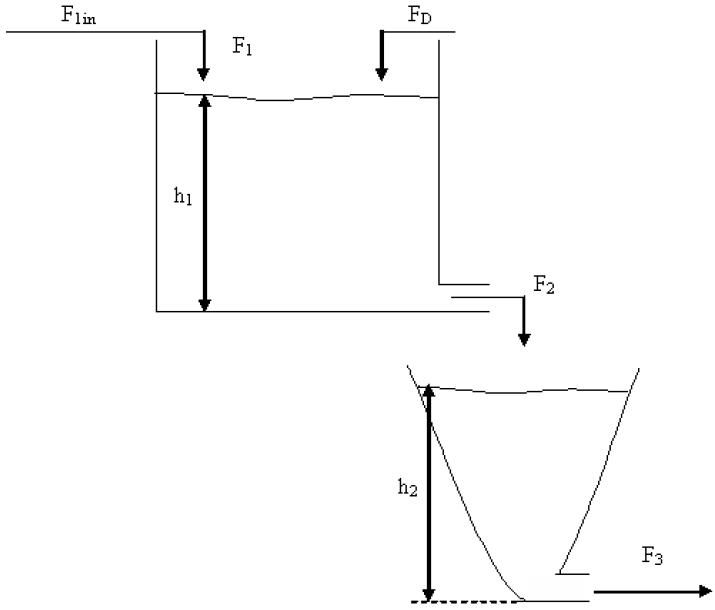
\includegraphics[width=0.8\textwidth]{pictures/schemat}
\caption{Obiekt regulacji automatycznej.}
\label{schemat}
\end{figure}

Wartością sterującą był dopływ $F_{1in}$ natomiast zakłóceniem - $F_D$. Z kolei wyjściem - wartością regulowaną - wysokość cieczy w drugim zbiorniku $h_2$. W pierwszej kolejności dokonano identyfikacji modelu, sprawdzono jego nieliniowość i dobrano odpowiedni rząd dynamiki modelu liniowego.
\section{Algorytmy regulacji predykcyjnej}
Do lat 70. ubiegłego wieku warstwa regulacji bezpośredniej w warstwowej strukturze sterowania (Rys. \ref{warstwy}) zapewniała przede wszystkim niezawodność \cite{120}. Dominowały wówczas algorytmy PID, natomiast rozwój optymalizacji postawił nowe wymagania przed układami regulacji \cite{160}. Okazało się bowiem, że skuteczna regulacja podczas optymalizacji punktu pracy przynosi duże korzyści ekonomiczne. To można było osiągnąć dzięki wprowadzeniu nowej grupy algorytmów - algorytmów regulacji predykcyjnej z przesuwnym horyzontem, zwanym też zasadą sterowania repetycyjnego \cite{160}. Pozwoliły po raz pierwszy rozwiązać problem uwzględnienia ograniczeń sygnałów sterujących.

\begin{figure}[h!]
\centering
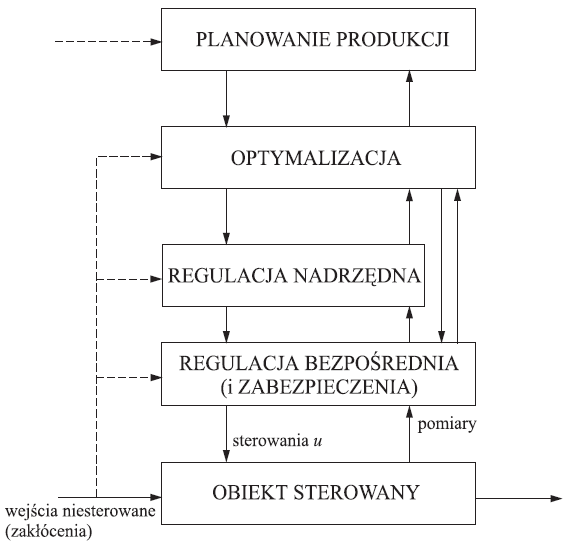
\includegraphics[width=0.5\textwidth]{pictures/warstwy}
\caption{Warstwowa struktura sterowania \cite{121}.}
\label{warstwy}
\end{figure}

W każdej chwili próbkowania, dysponując dynamicznym modele obiektu, pomiarami sygnałów procesowych oraz znaną lub założoną trajektorią wyjść zadanych wyznaczana jest sekwencja przyszłych wartości sygnału sterującego przez optymalizację funkcji celu zdefiniowanej na horyzoncie predykcji \cite{40}.

Najczęściej spotykana postać funkcji kryterialnej wygląda następująco:
\begin{equation}
J(k) = \min_{\Delta U(k)} \quad \{\sum_{p=1}^N (y^{zad}(k+p|k) - \hat{y}(k+p|k))^2 + \lambda \sum_{p=0}^{N_u} (\Delta u(k+p|k))^2\}
\end{equation}

przy ograniczeniach:

\begin{equation}
\begin{aligned}
u^{min} \quad &\leq& u(k+p|k) \quad &\leq& u^{max} \\
-\Delta u^{max} \quad &\leq& \Delta u(k+p|k) \quad &\leq& \Delta u^{max} \\
y^{min} \quad &\leq& \hat{y}(k+p|k) \quad &\leq& y^{max}
\end{aligned}
\end{equation}

\newpage

Wskaźnik jakości dostarcza informacji jakie wyniki powinien generować algorytm: uchyby regulacji muszą być jak najmniejsze, natomiast przyrosty sterowania nie powinny przyjmować dużych wartości, a ponadto korygowane są tzw. parametrem kary. Wyeliminowanie tego składnika ($\lambda = 0$) generuje przebiegi sygnału sterującego o dużych amplitudach i przyrostach, często niemożliwych do fizycznej realizacji. \\
Ograniczenia nałożone na sygnał sterujący związane są z uwarunkowaniami technologicznymi urządzeń wykonawczych, natomiast ograniczenia na sygnały wyjściowe służą spełnieniu norm technologicznych, ekonomicznych, a także zyskujących na coraz większym znaczeniu ekologicznych. Ogólna zasada regulacji predykcyjnej została zaprezentowana na Rys. \ref{mpc}

\begin{figure}[h!]
\centering
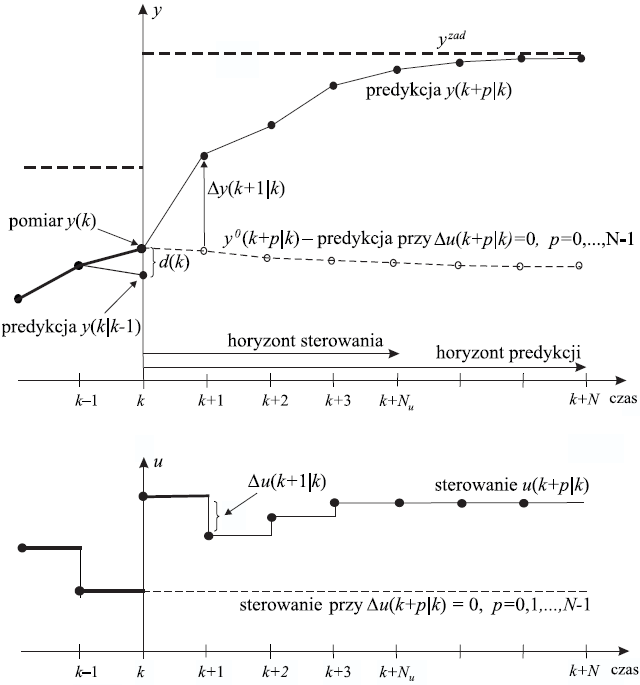
\includegraphics[width=0.65\textwidth]{pictures/mpc}
\caption{Zasada działania regulacji predykcyjnej \cite{122}.}
\label{mpc}
\end{figure}

Przedstawione przebiegi zawierają kilka istotnych aspektów, które warto opatrzeć komentarzem:
\begin{itemize}
\item[•] $y^{zad}$ - trajektoria sygnału zadanego, przyjmowana jako wartość stała na horyzoncie predykcji\footnote{Najczęściej zakładana jest stała trajektoria zadana, natomiast w niektórych dziedzinach, np. robotyka, dopuszcza się uwzględnienie zmian trajektorii zadanej w celu uprzedniego reagowania na jej zmiany.}
\item[•] $\Delta y(k+p|k)$ - prognozowana trajektoria odpowiedzi wymuszonej zależna tylko od zmiennych decyzyjnych - przyszłych przyrostów sterowań
\item[•] $y^0(k+p|k)$ - przewidywana odpowiedź swobodna, czyli wartości odpowiadające sytuacji, w której na całym horyzont predykcji $N$ utrzymywana byłaby wartość sterowania z chwili poprzedniej $u(k-1)$
\item[•] $\Delta u(k+p|k)$ - kolejne przyrosty sterowania wyznaczane na horyzoncie sterowania $N_u$
\end{itemize}

Na tej podstawie oraz korzystając z zasady superpozycji można zapisać:
\begin{equation}
y(k+p|k) = y^0(k+p|k) + \Delta y(k+p|k) \quad \quad p = 1 ... N
\end{equation}

\newpage

Zasada regulacji predykcyjnej jest dość uniwersalna co pozwoliło na wykształcenie kilku dominujących algorytmów, takich jak:
\begin{itemize}
\item[•] DMC (\textit{Dynamic Matrix Control}) - algorytm predykcyjny wykorzystujący model liniowy w postaci dyskretnych odpowiedzi skokowych
\item[•] GPC (\textit{Generalized Predictive Control}) - algorytm predykcyjny wykorzystujący model liniowy w postaci dyskretnych równań różnicowych
\item[•] MPCS (\textit{Model Predictive Control with State-space model}) - algorytm predykcyjny wykorzystujący w swoim opisie równania stanu
\item[•] MPHC (\textit{Model Predictive Heuristic Control}) - algorytm predykcyjny wykorzystujący model liniowy w postaci odpowiedzi impulsowej
\end{itemize}

Ze względu na praktyczną naturę algorytmu DMC do dalszych rozważań postanowiono przyjąć właśnie ten algorytm.

\section{Dynamic Matrix Control}
Algorytm DMC pierwszy raz został zaimplementowany przez grupę Shell Oil w latach \\ 70 XXw. Na tamten czas dało im to ogromną przewagę w branży petrochemicznej, a sam algorytm dzięki bezpośredniemu praktycznemu zastosowaniu stał się bardziej popularny. Algorytm ten zasadę swojego działania opiera na odpowiedzi skokowej, co wg autora \cite{120} stanowi jeden z najskuteczniejszych form identyfikacji obiektu. \\
Na Rys. \ref{step_response} przedstawiono przykład odpowiedzi skokowej na wymuszenie jednostkowe, zaprezentowane na horyzoncie dynamiki, czyli czas po którym wartość odpowiedzi skokowej można uznać za ustaloną, tj.
\begin{equation}
s_k = s_{k+1} = s_{k+2} = ... = s_D = s_{\infty}
\end{equation} 

\begin{figure}[h!]
\centering
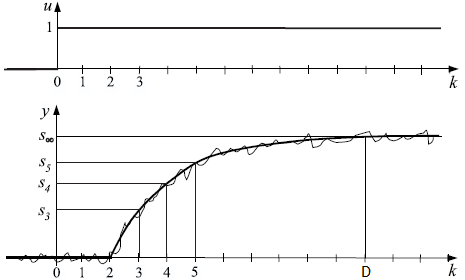
\includegraphics[width=0.75\textwidth]{pictures/step_response}
\caption{Odpowiedź skokowa \cite{123}.}
\label{step_response}
\end{figure}

Korzystając z zasady superpozycji, dla każdej chwili dyskretnej $k+p$, można zatem zapisać:

\begin{equation}
y^{mod}(k+p|k) = y^{mod}(0) + \sum_{j=1}^{k+p} s(j) \Delta u(k+p-j)
\end{equation}

\newpage

Z kolei wartość przewidywanej trajektorii wyjść można zapisać jako suma wartości modelu i~zakłócenia sprowadzonego do wyjścia:

\begin{equation}
\hat{y}(k+p|k) = y^{mod}(k+p|k) + d(k+p|k)
\end{equation} 

\noindent gdzie zakłócenie $d(k)$ jest równe różnicy między pomiarem wyjścia w chwili $k$, a wartością obliczoną z modelu w chwili $k-1$:

\begin{equation}
d(k) = y(k) - y^{mod}(k|k-1)
\end{equation}

\noindent natomiast ogólnie przejętą praktyką jest przyjmowanie modelu zakłóceń typu DMC, tj.

\begin{equation}
d(k+1|k) = d(k+2|k) = ... = d(k+N|k) = d(k)
\end{equation}

Takie założenia pozwalają na sformułowanie wyjściowej postaci trajektorii prognozowanej w algorytmie DMC:

\begin{equation}
\left\{
\begin{aligned}
\hat{y}(k+p|k) &= y^0(k+p|k) + \Delta y(k+p|k) \\
y^0(k+p|k) &= y(k) + \sum_{j=1}^k (s(j+p) - s(j))\Delta u(k-j)  \\
\Delta y(k+p|k) &= \sum_{j=1}^p s(j) \Delta u(k+p-j)
\end{aligned}
\right.
\label{prognoza}
\end{equation}

Zatem w ogólności można zapisać trajektoria prognozowana jest sumą odpowiedzi swobodnej i wymuszonej. Algorytm DMC występuje w wersji analitycznej bez oraz z rzutowaniem na ograniczenia oraz w wersji numerycznej, uwzględniającej te ograniczenia. 

\subsection{Algorytm DMC w wersji analitycznej}
Do sformułowania prawa regulacji w wersji analitycznej, w postaci wektorowej niezbędne jest zdefiniowanie wektorów postaci:

\begin{equation}
\begin{aligned}
Y^{zad} = \begin{bmatrix}
y^{zad}(k+1|k) \\ \vdots \\ y^{zad}(k+N|k)
\end{bmatrix}_{Nx1}, \quad
\hat{Y} = \begin{bmatrix}
\hat{y}(k+1|k) \\ \vdots \\ \hat{y}(k+N|k)
\end{bmatrix}_{Nx1}, \quad
\Delta U(k) = \begin{bmatrix}
\Delta u(k|k) \\ \vdots \\ \Delta u(k+N_u-1|k)
\end{bmatrix}_{N_ux1}
\end{aligned}
\end{equation}

\noindent Oraz macierzy wagowych:

\begin{equation}
\begin{aligned}
\Psi = \begin{bmatrix}
\psi_1 & & \\ & \ddots & \\ & & \psi_N
\end{bmatrix}_{NxN}, \quad
\Lambda = \begin{bmatrix}
\lambda_0 & & \\ & \ddots & \\ & & \lambda_{N_u-1}
\end{bmatrix}_{N_u x N_u}
\end{aligned}
\end{equation}

\noindent Tak zdefiniowane wektory pozwalają zapisać funkcję celu w postaci:

\begin{equation}
J(k) = \min_{\Delta U(k)} \{||Y^{zad} - \hat{Y}(k)||^2_\Psi + ||\Delta U(k)||^2_\Lambda \}
\label{cel}
\end{equation}

\noindent Odwołując się do równania \ref{prognoza} prognozowaną trajektorię wyjść w wersji macierzowo-wektorowej można zapisać w postaci:

\begin{equation}
\left\{
\begin{aligned}
\hat{Y} &= Y^0(k) + \Delta Y(k) \\
Y^0(k)& = Y(k) + M^P \Delta U^P(k) \\
\Delta Y(k) &= M \Delta U(k)
\end{aligned}
\right.
\end{equation}

\newpage

\noindent gdzie:
\begin{equation}
\begin{aligned}
&M^P = \begin{bmatrix}
s_2 - s_1 & s_3 - s_2 & \cdots & s_D - s_{D-1} \\
s_3 - s_1 & s_4 - s_2 & \cdots & s_D - s_{D-1} \\
\vdots & \vdots & \ddots & \vdots \\ 
s_{N+1} - s_1 & s_{N+2} - s_2 & \cdots & s_{N+D-1} - s_{D-1}
\end{bmatrix}_{Nx(D-1)} \\
&M = \begin{bmatrix}
s_1 & 0 & \cdots & 0 \\
s_2 & s_1 & \cdots & 0 \\ 
\vdots & \vdots & \ddots & \vdots \\
s_N & s_{N-1} & \cdots & s_{N-N_u+1} \\
\end{bmatrix}_{NxN_u}, \quad
\Delta U^P(k) = \begin{bmatrix}
\Delta u(k-1) \\ \vdots \\ \Delta u(k-D+1)
\end{bmatrix}_{(D-1)x1}
\end{aligned}
\end{equation}

\noindent Wektor $\Delta U^P(k)$ opisuje wartości przyrostów sterowań z poprzednich chwil, natomiast macierz $M$ nazywana jest macierzą dynamiczną. Uwzględniając postać funkcji kryterialnej (\ref{cel}) oraz przyjmując odpowiednie założenia $\Psi \geq 0$ oraz $\Lambda \geq 0$ wektor kolejnych przerostów sterowań dany jest wzorem:

\begin{equation}
\Delta U(k) = K(Y^{zad} - Y^0)
\label{delta_u}
\end{equation}

\noindent gdzie

\begin{equation}
K = (M^T \Psi M  + \Lambda)^{-1} M^T \Psi
\end{equation}

\noindent Zważywszy na fakt, że w każdej iteracji algorytmu wykorzystywany jest tylko pierwsza z wyznaczonych wartości przyrostów sterowań, równanie \ref{delta_u} można uprościć i zapisać w postaci:

\begin{equation}
\Delta u(k) = \bar{K_1} (Y^{zad} - Y^0(k))
\label{u_anal}
\end{equation}

\noindent gdzie $\bar{K_1}$ jest pierwszym wierszem macierzy $K$. Równanie \ref{u_anal} opisuje analityczną postać algorytmu DMC. Kolejnym istotnym aspektem jest rzutowanie wyznaczanych wartości na ograniczenia:

\begin{equation}
\begin{aligned}
u^{min} \quad &\leq& u(k+1|k) \quad &\leq& u^{max} \\
-\Delta u^{max} \quad &\leq& \Delta u(k|k) \quad &\leq& \Delta u^{max} \\
y^{min} \quad &\leq& \hat{y}(k|k) \quad &\leq& y^{max}
\end{aligned}
\end{equation}

Wersja analityczna DMC znajduje zastosowanie w praktyce, szczególnie w systemach liniowych o niewielkiej liczbie zmiennych sterowania i ograniczeń. Jednak w bardziej złożonych przypadkach, zwłaszcza z dużymi układami wielowymiarowymi lub w systemach nieliniowych, częściej stosuje się wersję numeryczną.

\subsection{Algorytm DMC w wersji numerycznej}
Kwadratowa funkcja kryterialna - dzięki zastosowaniu modelu liniowego do predykcji - umożliwia rozwiązanie zadania minimalizacji w sposób analityczny, ale również numeryczny. Optymalizacja numeryczna ma tę przewagę, że pozwala uwzględnić ograniczenia nałożone na sygnał sterujący \cite{160}, tzn. w każdej iteracji wyznaczany jest wektor przyszłych sterowań w wyniku rozwiązania następującego zadania optymalizacji w postaci standardowej:

\begin{equation}
min \{J(x) = \frac{1}{2} x^T Hx + f^T x\} \\
\end{equation} 

\noindent przy ograniczeniach:

\begin{equation}
\begin{aligned}
x_{min} \leq &x \leq x_{max} \\
Ax &\leq b
\end{aligned}
\end{equation}

\newpage

\noindent gdzie:

\begin{equation}
\begin{aligned}
x &= \Delta U(k), \quad x_{min} = -\Delta U_{max}, \quad x_max = \Delta U_max \\
H &= 2(M^T \Psi M + \Lambda) \\
f &= -2M^T \Psi (Y^{zad}(k) - Y^0(k)) \\
A &= \begin{bmatrix}
-J \\ J \\ -M \\ M
\end{bmatrix}, \quad
b = \begin{bmatrix}
-U_{min} + U(k-1) \\ U_{max} - U(k-1) \\ 
-Y_{min} + Y^0(k) \\ Y_{max} - Y^0(k) 	 	
\end{bmatrix} \\
J &= \mathbb{I}_{N_u x N_u}, \quad Y_{min} = [y_{min}, ..., y_{min}]^T, \quad Y_{max} = [y_{max}, ..., y_{max}]^T
\end{aligned}
\end{equation}

Działanie regulatora DMC z ograniczeniami zostało przedstawione w pracy \cite{50}, w której autorzy dokonali szereg testów sprawdzających wpływ przeprowadzanej optymalizacji w każdym kroku na jakość regulacji.

\subsection{Inne warianty DMC}
Zastosowanie algorytmów predykcyjnych w latach 70. ubiegłego stulecia pokazało jak duże korzyści - nie tylko w aspekcie jakości regulacji, ale także ekonomicznych - może przynieść ich wdrożenie do obiektu sterowania. Wówczas ten fakt spowodował dynamiczny rozwój tych algorytmów, czego efektem są m.in. algorytmy wykorzystujące nieliniowe modele obiektów:
\begin{itemize}
\item[-] Algorytm DMC z sukcesywną linearyzacją (DMC-SL)
\item[-] Algorytm DMC z nieliniową optymalizacją (DMC-NO)
\item[-] Algorytm DMC z nieliniową predykcją i linearyzacją (DMC-NPL)
\end{itemize}

\begin{description}
\item \textbf{DMC-SL} \\
Algorytm podstawowy, korzystający z modelu liniowego często może okazać się niewystarczający, np. gdy obiekt wykazuje silną nieliniowość. Dużą poprawę, tj. minimalizację błędów linearyzacji, można osiągnąć implementując algorytm predykcyjny z sukcesywną linearyzacją. W każdej iteracji, dokonywana jest linearyzacja modelu nieliniowego w punkcie pracy, w którym aktualnie znajduje się obiekt. Następnie na podstawie modelu liniowego wyznaczana jest odpowiedź skokowa oraz formowana jest macierz dynamiczna \cite{170, 120}. Okazuje się, że linearyzacja modelu nie jest wymagana w każdym kroku, co zaprezentował autor \cite{30}. Jeśli zmiany między kolejnymi wartościami predykcji nie są duże, można korzystać z uprzednio wyznaczonego modelu liniowego.

\item \textbf{DMC-NPL} \\
Algorytm DMC z nieliniową predykcją i linearyzacją jest zmodyfikowaną wersją algorytmu wykorzystującą sukcesywną linearyzacji. W tym przypadku bowiem odpowiedź swobodna jest wyznaczana na podstawie modelu nieliniowego, natomiast linearyzacja służy wyznaczeniu odpowiedzi skokowej i sformułowania macierzy dynamicznej - podobnie jak w DMC-SL. Marginalizacja wpływu modelu liniowego na proces przynosi poprawę szczególnie w przypadkach gdy regulowany obiekt wykazuję silną nieliniowość charakteryzuje się szybkim przechodzenie do odległych punktów równowagi, np. po wystąpieniu silnych zakłóceń czy tez przy uruchamianiu lub wyłączaniu procesów \cite{170, 120}.

\item \textbf{DMC-NO} \\
Algorytm ten zaliczany jest do grupy algorytmów z nieliniową optymalizacją. Wykorzystuje pełny nieliniowy model procesu do predykcji. Prostota koncepcji i jakość regulacji na najwyższym poziomie nie są jednak w stanie zrekompensować istotnych wad tego podejścia, mianowicie złożoność obliczeniowa oraz fakt, że nie istnieją algorytmy rozwiązujące nieliniowy problem optymalizacji w możliwym do oszacowania czasie eliminują algorytm DMC-NO z praktycznego użycia \cite{170}.
\end{description}
\chapter{Regulacja rozmyta}
Tytułowy typ regulacji zrywa ze standardową procedurą podejmowania decyzji w sposób binarny, tzn. $1 / 0$ \cite{40}. Na Rys. \ref{crisp} przedstawiono standardową funkcję przynależności do zbioru, którą można opisać wzorem:

\begin{equation}
\mu_C = \begin{cases}
1, \quad x \in [a, b] \\
0, \quad x \notin [a, b]
\end{cases}
\end{equation}

\begin{figure}[h!]
\centering
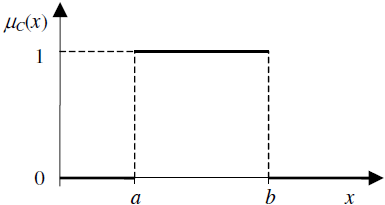
\includegraphics[width=0.5\textwidth]{pictures/crisp}
\caption{Funkcja przynależności zbioru ostrego.}
\label{crisp}
\end{figure}

Natomiast istota wnioskowania rozmytego polega na zgromadzeniu wiedzy eksperckiej, operatora procesu, wspartej odpowiedzią skokową obiektu, które pozwolą na sformułowanie zbiorów rozmytych (Rys. \ref{fuzzy_set}) oraz bazy reguł definiującej regulator rozmyty \cite{160, 170}. Funkcja przynależności zbioru rozmytego została zaprezentowana na Rys. \ref{fuzzy} i w tym przypadku dana jest wzorem:

\begin{equation}
\mu_C = \begin{cases}
0,& \quad x \leq c \vee x \geq f \\
\frac{x-c}{d-c},& \quad c \leq x \leq d \\ 
1,& \quad d \leq x \leq e \\
\frac{f-x}{f-e},& \quad e \leq x \leq f
\end{cases}
\end{equation}

\begin{figure}[h!]
\centering
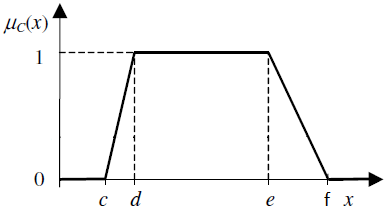
\includegraphics[width=0.5\textwidth]{pictures/fuzzy}
\caption{Funkcja przynależności zbioru rozmytego.}
\label{fuzzy}
\end{figure}

\newpage

\noindent Zmienne z odcinków $[c,d]$ oraz $[e,f]$ przyjmują wartości z przedziału $[0,1]$, w tym sensie granice zbioru przynależności są rozmyte. Natomiast wartość funkcji przynależności do zbioru określana jest stopniem przynależności. Należy w tym miejscu zwrócić uwagę na kształty funkcji przynależności. Funkcje trapezowe bądź trójkątne proste w swym zapisie, nie są różniczkowalne. Aspekt ten jest o tyle istotny, że zapewnia stabilność, zwiększa dokładność w systemach sterowania rozmytego, a także jest niezbędny podczas uczenia maszynowego, wykorzystującego metody gradientowe. Dlatego w wielu zastosowaniach przyjęło się korzystanie z innych kształtów funkcji przynależności, zapewniających różniczkowalność, takich jak: gaussowskie, dzwonowe, sigmoidalne.

\begin{figure}[h!]
\centering
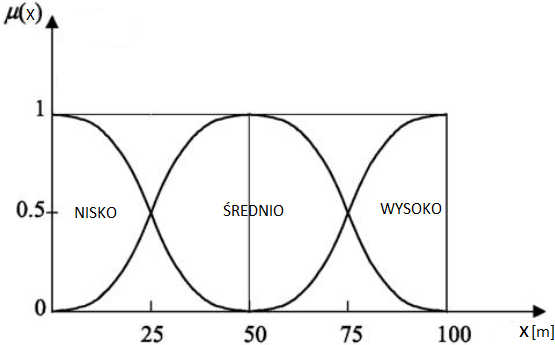
\includegraphics[width=0.75\textwidth]{pictures/fuzzy_set}
\caption{Przykładowe zbiory rozmyte.}
\label{fuzzy_set}
\end{figure}

Ważną kwestią w rozumieniu systemów rozmytych, jest pośrednik między zmienną numeryczną, a zmienną symboliczną - zmienna lingwistyczna. Na Rys. \ref{fuzzy_set} przedstawiono rozmycie zmiennej "wysokość", która przyjmuje trzy wartości: "nisko", "średnio", "wysoko" i tak można zauważyć, że wartość numeryczna $75m$ ze stopniem przynależności $0,5$ należy do zbiorów "średnio" oraz "wysoko" \cite{90, 120, 130}. \\
Po rozmyciu zmiennej lingwistycznej, określeniu stopni przynależności danych wartości do poszczególnych zbiorów pozostaje jeszcze zdefiniowanie bazy wiedzy, czyli tzw. zbioru reguł. Każda reguła składa się z części warunkowej, zwanej poprzednikiem oraz konsekwencji, określanej następnikiem. Ogólna struktura reguły w rozumieniu systemów rozmytych przyjmuje postać:

\begin{equation}
\text{JEŚLI } <poprzednik> \text{ TO } <następnik> 
\end{equation}

Poprzedniki reguł w najprostszym przypadku mogą zawierać pojedynczy warunek w innej sytuacji mogą składać się z kilku prostych warunków połączonych operacjami logicznymi (i, lub, nie).

\begin{itemize}
\item[•] warunek prosty: $\text{JEŚLI } x \text{ jest } A \text{ TO } <następnik>$ \\
\item[•] warunek złożony: $\text{JEŚLI } x_1 \text{ jest } A_1 \text{ lub } x_2 \text{ jest } A_2 \text{ i } x_3 \text{ nie jest } A_3 \text{ TO } <następnik>$ \\
\end{itemize}

\newpage

W przypadku następników reguł wyróżnić można ich trzy postaci:

\begin{enumerate}
\item Następnik ostry
\begin{equation}
\text{JEŚLI } <poprzednik> \text{ TO } y = y_a
\end{equation}

\item Następnik rozmyty 
\begin{equation}
\text{JEŚLI } <poprzednik> \text{ TO } y \text{ jest } Y_a
\end{equation}

\item Następnik funkcyjny
\begin{equation}
\text{JEŚLI } <poprzednik> \text{ TO } y = f(x_1, x_2, ... , x_k)
\end{equation}
\end{enumerate}

\noindent Szczególnie istotne oraz wykorzystywane w praktyce są dwie ostatnie wymienione metody. Następniki w postaci zbiorów rozmytych są z powodzeniem wykorzystywane w modelach Mamdaniego \cite{170, 90}, gdzie wykorzystując wiedzę eksperta można z dużą dokładnością sterować obiektem regulacji w sposób rozmyty. Częstą praktyką w tym podejściu jest budowanie tablicy decyzyjnej, która w stosunkowo prosty i przejrzysty sposób redukuję bazę reguł do tabeli \cite{170}. \\
W kontekście niniejszej pracy skupiono się przede wszystkim na następnikach funkcyjnych opisujących modele Takagi - Sugeno, którym poświęcono następny rozdział. 

\section{Modele Takagi-Sugeno}
Projektowanie modeli Takagi-Sugeno składa się z następujących etapów:

\begin{enumerate}
\item Obliczenie poziomów aktywacji reguł
\item Wyznaczenie konkluzji - obliczenie wartości następników funkcyjnych poszczególnych reguł
\item Wyznaczenie konkluzji końcowej - zsumowanie wartości następników funkcyjnych - ważone i normowane - z uwzględnieniem sił odpalenia reguł, co opisuje wzór \ref{wniosek}.
\end{enumerate}

\begin{equation}
y = \frac{\sum_{j=1}^r w^j y^j}{\sum_{j=1}^r w^j}
\label{wniosek}
\end{equation}

\noindent gdzie:
\begin{itemize}
\item[•] $r$ - liczba reguł
\item[•] $w^j$ - siły odpalenia poszczególnych reguł
\item[•] $y^j$ - wartości odpowiednich następników funkcyjnych
\end{itemize}

Ogólnie modele rozmyte służą do aproksymacji funkcji nieliniowych stąd w przypadku modeli Takagi-Sugeno następniki funkcyjne występują najczęściej w postaci funkcji wielomianowych pierwszego rzędu \cite{160, 170}:

\begin{equation}
\text{JEŚLI } <poprzednik> \text{ TO } y = a_0 + \sum_{j=1}^n a_jx_j
\end{equation} 

Natomiast w pracy skupiono się jakie korzyści może przynieść zastosowanie nieliniowych - hiperbolicznych - następników. Według autorów \cite{80} pozwala to na zmniejszenie liczby zbiorów rozmytych, a tym samym reguł.

\newpage

\section{Podejście PDC}
Podejście PDC (\textit{Parallel Distributed Combensation}) zakłada dedukcję regulatora za pomocą modelu Takagi-Sugeno obiektu. Istota równoległej kompensacji rozproszonej polega na dobraniu dla każdego następnika rozmytego lokalnego regulatora liniowego. Zatem w wyniku takiego podejścia otrzymuje się tyle regulatorów z ilu modeli lokalnych, opisujących obiekt w danych obszarze, składa się system rozmyty. Na początku zakłada się taką samą postać poprzedników jak w modelu obiektu, następnie w miarę potrzeby dostraja \cite{120, 170}. Struktura regulatora otrzymanego w wyniku zastosowania podejścia PDC została przedstawiona na Rys. \ref{pdc}.

\begin{figure}[h!]
\centering
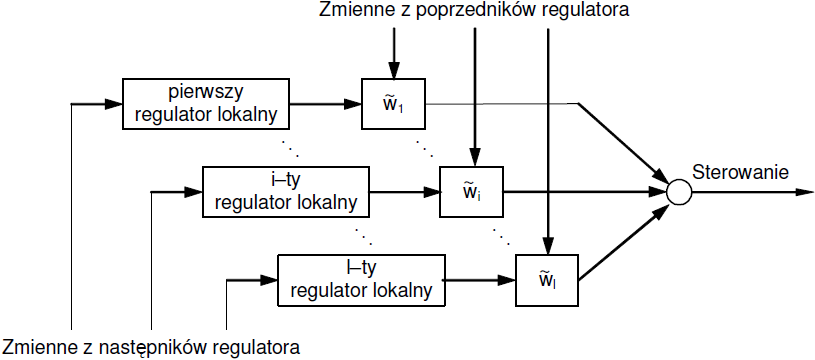
\includegraphics[width=0.75\textwidth]{pictures/pdc}
\caption{Struktura regulatora rozmytego otrzymanego podejściem PDC \cite{171}.}
\label{pdc}
\end{figure}
\chapter{Modele Hammersteina i Wienera}
Istotą stosowania modeli Hammersteina i Wienera jest rozdzielenie liniowej dynamiki od zakłóceń wprowadzanych przez statyczne nieliniowości. Mogę one występować na wejściu \\ (Rys. \ref{hamm}) bądź wyjściu (Rys. \ref{wien}) \cite{10}.
\vspace{0.5cm}
\begin{figure}[h!]
\centering
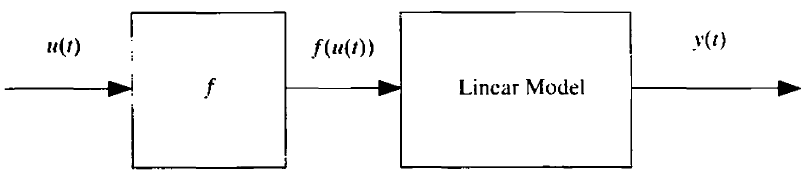
\includegraphics[width=\textwidth]{pictures/hammerstein}
\caption{Model Hammersteina \cite{21}.}
\label{hamm}

\vspace{0.5cm}

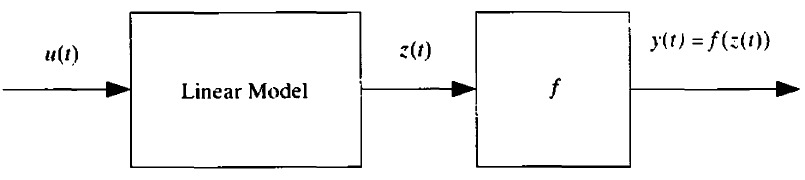
\includegraphics[width=\textwidth]{pictures/wiener}
\caption{Model Wienera \cite{21}.}
\label{wien}
\end{figure}

Modele te doskonale nadają się do identyfikacji systemów nieliniowych. Często w tym celu wykorzystywane są funkcje wielomianowe, sieci neuronowe czy systemy rozmyte \cite{150}.
\begin{thebibliography}{99}
\setstretch{1.5} % Ustawienie interlinii na 1.5

\bibitem{10} A. Janczak. \textit{Identification of Nonlinear Systems Using Neural Networks and Polynomial Models.} Zielona Góra, Springer, 2005.

\bibitem{20} L. Ljung. \textit{System Identification. Theory for the User,} wyd. 2. Szwecja, Prentice Hall, 1999.

\bibitem{21} L. Ljung. \textit{Above: A Harrunerstein model. Below: A Wiener model}, [ilustracja]. \\ W: \textit{System Identification. Theory for the User,} wyd. 2. Szwecja, Prentice Hall, 1999. 

\bibitem{150} M. Ławryńczuk. \textit{Modelowanie i identyfikacja}. Warszawa, 2022.

\bibitem{160} M. Ławryńczuk. \textit{Sterowanie procesów ciągłych}. Warszawa, 2022.

\bibitem{170} M. Ławryńczuk, P. Marusak. \textit{Sztuczna inteligencja w automatyce}. Warszawa, 2009–2018.

\bibitem{171} M. Ławryńczuk, P. Marusak. \textit{Regulator typu Takagi–Sugeno otrzymany za pomoca podejscia PDC}, [ilustracja]. W: \textit{Sztuczna inteligencja w automatyce}. Warszawa, 2009–2018.

\bibitem{30} J. M. Maciejowski. \textit{Predictive Control with Constraints.} Harlow, Prentice Hall, 2002.

\bibitem{35} K. Malinowski, P. Tatjewski. \textit{Podstawy Automatyki}, wyd. 2. Warszawa, 2016.

\bibitem{40} P. Marusak. \textit{Regulacja predykcyjna obiektów nieliniowych z zastosowaniem techniki DMC i modelowania rozmytego}. Warszawa, Wydział Elektroniki i Technik Informacyjnych, 2002.

\bibitem{50} P. Marusak, J. Pułaczewski, P. Tatjewski. \textit{Algorytmy DMC z uwzględnieniem ograniczeń sterowania}, vol. 1.  Opole, 1999.

\bibitem{60} P. Marusak, P. Tatjewski. \textit{Fuzzy Dynamic Matrix Control algorithms for nonlinear plants}, vol. 2. Międzyzdroje, 2000.

\bibitem{70} K. Mehran. \textit{Takagi-Sugeno Fuzzy Modeling for Process Control}. Newcastle, 2008.

\bibitem{80} H. Moodi, M. Farrokhi. \textit{Robust observer-based controller design for Takagi–Sugeno systems with nonlinear consequent parts}. W: \textit{Fuzzy Sets and Systems}. Amsterdam, Elsevier B.V., 2015.\\ Nr 273, s. 141-154, ISNN 0165-0114.

\bibitem{90} K. Rykaczewski. \textit{Systemy rozmyte i ich zastosowania}. Toruń, 2006.

\bibitem{120} P. Tatjewski. \textit{Sterowanie zaawansowane obiektów przemysłowych. Struktury i algorytmy}.\\ Warszawa, Akademicka Oficyna Wydawnicza EXIT, 2016.

\bibitem{121} P. Tatjewski. \textit{Warstwowa struktura sterowania obiektem przemysłowym}, [ilustracja].\\ W: \textit{Sterowanie zaawansowane obiektów przemysłowych. Struktury i algorytmy}.\\ Warszawa, Akademicka Oficyna Wydawnicza EXIT, 2016.

\bibitem{122} P. Tatjewski. \textit{Zasada regulacji predykcyjnej}, [ilustracja].\\ W: \textit{Sterowanie zaawansowane obiektów przemysłowych. Struktury i algorytmy}.\\ Warszawa, Akademicka Oficyna Wydawnicza EXIT, 2016.

\newpage

\bibitem{123} P. Tatjewski. \textit{Przykład odpowiedzi wyjscia obiektu y na skok sterowania u}, [ilustracja].\\ W: \textit{Sterowanie zaawansowane obiektów przemysłowych. Struktury i algorytmy}.\\ Warszawa, Akademicka Oficyna Wydawnicza EXIT, 2016.

\bibitem{130} A. Piegat. \textit{Modelowanie i sterowanie rozmyte}.\\ Warszawa, Akademicka Oficyna Wydawnicza EXIT, 1999.

\end{thebibliography}

\listoffigures
\end{document}